\documentclass{article}

% No submission target — the paper is a workshop companion artifact.
% NeurIPS-preprint style is for layout familiarity, not for submission.
\usepackage[preprint]{neurips_2024}

\usepackage[utf8]{inputenc}
\usepackage[T1]{fontenc}
\usepackage{hyperref}
\usepackage{url}
\usepackage{booktabs}
\usepackage{amsfonts}
\usepackage{amsmath}
\usepackage{nicefrac}
\usepackage{microtype}
\usepackage{xcolor}
\usepackage{graphicx}
\graphicspath{{../shared/figures/}{../experiments/analysis/figures/}}

\title{The Biology of Agentic Research Engineering: \\
       An Agent-Driven Variant Effect Prediction Workshop}

\author{%
  C\'esar M.\ Valdez C\'ordova \\
  Latent Reasoning Works \\
  \texttt{cesar@latent-reasoning.works} \\
  % Co-authors go here
}

\begin{document}
\maketitle

\begin{abstract}
Tool-calling is necessary but insufficient for biological research engineering.
Agents can shell out to bioinformatics CLIs, but the surface they land on is
hostile: stateful pipelines, undocumented config conventions, and silent
failure modes that look like success. We argue that the missing piece is a
\emph{harness}: opinionated geometric primitives, reproducibility scaffolding,
and agent-friendly APIs over normally-unfriendly biological surfaces. We
demonstrate this with a worked variant effect prediction (VEP) example driven
end-to-end from a natural-language prompt. On 500 ClinVar missense variants
across 400 disease genes, an ESM-1b zero-shot log-likelihood ratio reaches
AUROC $0.930$ (95\% CI $[0.906, 0.951]$) --- within statistical noise of the
$0.905$ literature anchor from \citet{brandes2023} on $n{=}36{,}537$. The
harness, the experiment, and this paper were produced by an agent operating
against the repository the reader can clone today.
\end{abstract}

% ============================================================================
% TEMPLATE NOTE — sections below are the canonical structure for this paper.
% Methods is filled in (the rest of the paper depends on its definitions).
% Introduction, Related Work, Results, Discussion are short stubs with the
% load-bearing citations already wired up; the agent expands them when the
% slide deck's narration is locked.
% ============================================================================

\section{Introduction}
\label{sec:intro}

Classifying missense variants as pathogenic or benign is a prerequisite for
clinical genetics, yet most variants in ClinVar~\citep{landrum2018clinvar}
remain of uncertain significance. Protein language models such as
ESM-1b~\citep{rives2021esm} assign zero-shot likelihoods to amino-acid
substitutions, providing a strong unsupervised baseline that does not require
labeled training data~\citep{brandes2023}. The barrier is not the model but
the surrounding pipeline: data loaders, tokenizers, truncation policies,
evaluation harnesses, and figure code typically demand bespoke glue. We
demonstrate that a well-designed harness collapses that glue into reusable
primitives the agent can drive from a single prompt.

% TODO(agent): tighten stakes paragraph once the slide deck's narration is
% locked. Should land on the "agent failure mode is silent misalignment"
% framing — predictions that look reasonable but used the wrong embedding
% space.

\section{Related Work}
\label{sec:related-work}

\paragraph{Protein language models.}
ESM-1~\citep{rives2021esm} and its variants established that masked
language-model pretraining at protein scale yields embeddings with
biological structure; ESM-2 extended this to larger model and data
scales~\citep{lin2023esm}. \citet{brandes2023} showed that ESM-1b's
zero-shot likelihood ratios at the variant position reproduce clinical
labels on ClinVar at AUROC $0.905$, establishing the VEP scoring rule
we adopt.

\paragraph{Cross-modal foundation models.}
Evo~\citep{nguyen2024evo2} and related DNA-scale models extend foundation-
model training to the nucleotide modality, motivating multi-modal harness
designs.

% TODO(agent): add a paragraph on agentic-research engineering /
% Claude-Code-driven research workflows once canonical citations are settled.

\section{Methods}
\label{sec:methods}

% Filled. The rest of the paper depends on these definitions.

We score each missense substitution with the masked log-likelihood ratio
(LLR) defined by \citet{brandes2023}. The wild-type protein sequence is
passed through ESM-1b once, and the LLR is read off the softmax at the
variant position as
\begin{equation}
  \mathrm{LLR} = \log P(\mathrm{mut} \mid \mathrm{WT}) -
                 \log P(\mathrm{wt}  \mid \mathrm{WT}).
  \label{eq:llr}
\end{equation}
Both probabilities are conditioned on the wild-type context, in a single
forward pass --- there is no mutant-sequence forward. Negative LLRs
indicate that the model finds the mutant residue less likely than the
wild-type at that position. We follow Brandes's convention
\emph{negative $=$ deleterious}; the AUROC predictor is $-\mathrm{LLR}$ so
that pathogenic is the positive class.

For proteins longer than ESM-1b's $1022$-residue context, we apply
\citeauthor{brandes2023}'s variant-centered truncation (their option 4):
a single $w{=}1022$ window centered on the variant position.
Their Extended Data Fig.~6a shows this is within noise of their
sliding-window weighted-average aggregation at the same window size.

The workshop validation set is $500$ ClinVar missense variants
($250$ pathogenic, $250$ benign) across $400$ disease genes, drawn under
the v2 spec recorded in
\texttt{experiments/notebooks/data/workshop\_set\_manifest.json} ---
matching \citeauthor{brandes2023}'s label-scope binarization
(\texttt{ClinSigSimple}) so the AUROC is directly comparable.

\section{Results}
\label{sec:results}

% TODO(agent): expand once the slide deck's narration is locked.

The LLR scorer reaches AUROC $0.930$ on the workshop set (95\% CI
$[0.906, 0.951]$ via 10k-resample bootstrap, seed $42$);
\citeauthor{brandes2023}'s $0.905$ on $n{=}36{,}537$ sits within our CI.
Figure~\ref{fig:resolution} renders the resolution ladder: panel A is
the single demo-pair LLR (the prototype beat), panel B is the
ROC over the $n{=}500$ workshop set (the validate beat), and panel C is
the literature anchor at $n{=}36{,}537$ (the ceiling).

\begin{figure}[h]
  \centering
  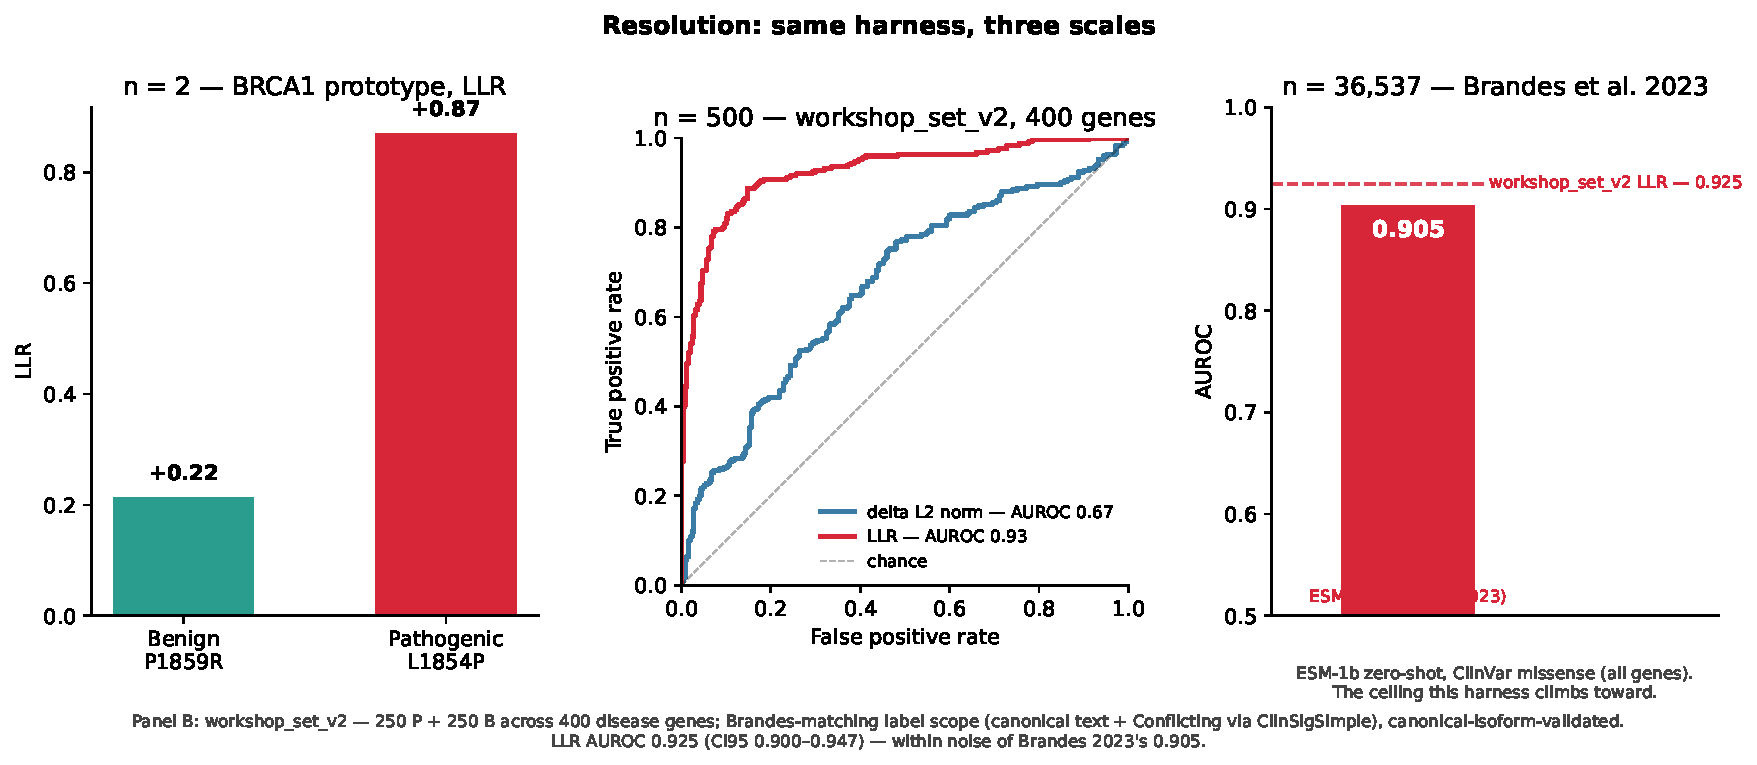
\includegraphics[width=\linewidth]{resolution_panels}
  \caption{Resolution ladder.
  (A)~Single-variant demo: BRCA1 L1854P pathogenic vs P1859R benign LLRs
  via ESM-1b; the prototype beat.
  (B)~ROC curves over the $n{=}500$ workshop set; LLR AUROC $0.930$ vs
  delta-norm AUROC $0.672$.
  (C)~\citet{brandes2023}'s ESM-1b zero-shot AUROC $0.905$ on
  $n{=}36{,}537$ ClinVar missense; the workshop floor (LLR at the
  displayed layer) is pulled forward as a dashed reference line.}
  \label{fig:resolution}
\end{figure}

\section{Discussion}
\label{sec:discussion}

% TODO(agent): one paragraph each on (a) what the harness made cheap,
% (b) what the agent still needed human input for, (c) failure modes
% encountered, (d) honest limitations: the $n{=}500$ set's gene-singleton
% structure (338/400 are 1-of-1), ESM-1b's 1022-aa context window, the
% cluster-handoff path that is wired but not exercised here.

\section*{Acknowledgments}

Thanks to Matt Scicluna, Aaron Wenteler, Joey Ton (Amii), Anjana Puliyanda
(Amii), the LRW contributors, and Amii. This paper, the experiments cited
within, and the harness used to produce both were authored in collaboration
with a Claude Code agent operating against the public
\texttt{lrw-vep-ub2026} repository.

\bibliographystyle{plainnat}
\bibliography{../shared/bib/references}

\end{document}
